\documentclass{ctexart}

%%%% Chinese support
%

%%%% Page geometry
\usepackage[
    a4paper,
    total={210mm,297mm},
    left=20mm,
    right=20mm,
    top=20mm,
    bottom=20mm,
  ]{geometry}            %

%%%% Math
\usepackage{amsmath}     %
\usepackage{siunitx}     % SI unit support

%%%% Caption
\usepackage{caption}
\captionsetup{belowskip=8pt,aboveskip=4pt}


%%%% Graph processing
\usepackage{graphicx}    % graph inclusion

%%%% Table processing
\usepackage{tabularx}
\usepackage{booktabs}    %
\usepackage{csvsimple}   % CSV table processing
\usepackage{multirow}    % multirow in table

%%%% Hyper reference
\usepackage[
    bookmarksnumbered=true,
    colorlinks=true,
    allcolors=blue,
  ]{hyperref}             %

%%%% Bibliography
\usepackage[
    backend=biber,
    style=numeric,
    citestyle=ieee,
    bibencoding=utf8,
  ]{biblatex}             %
\addbibresource{compact_debris_cfd.bib}

\usepackage{textcomp}

\title{龙卷风风场中块状飞射物的飞行特性:计算流体力学模拟}
\author{王勇}

\begin{document}
\maketitle
\begin{abstract}
本文主要通过计算流体力学方法模拟龙卷风风场中块状飞射物的飞行特性。
首先利用ANSYS Fluent 计算流体力学软件模拟龙卷风风场,并与多普勒雷达实测龙卷风风场对比,以检验模拟结果的正确性。
然后介绍ANSYS Fluent的离散相模型,以模拟在龙卷风风场中块状飞射物的运动。
最后通过一个算例比较本文的模拟方法与解析方法的结果。
\end{abstract}

\section{龙卷风的数值模拟}
实际情况中龙卷风的风场结构十分复杂,不仅有着单涡和多涡等多种形式,还具有一定的平移速度。
出于简化影响因素的考虑,本文仅模拟单涡形式的龙卷风,且假定龙卷风为定常风场。
并且部考虑龙卷风的平移运动,忽略地面粗糙度的影响。

\subsection{龙卷风发生装置}
本文模拟龙卷风的物理模型,是基于东京理工大学Matsui等人\cite{matsui2009}设计的实验室龙卷风模拟装置(见图\ref{fig:matsui_tornado_generator})。
为了模拟1998年5月30日多普勒雷达测得的美国南达科他州地区实际发生的一个龙卷风,本文采用全尺寸模型,调整了模型中各部分的尺寸参数,最后确定了龙卷风数值模型的物理发生装置\cite{tang2013}。
该发生装置的具体形式如图\ref{fig:tornado_generator}所示,模型各部分尺寸及参数设置见表\ref{tab:tornado_generator_parameters}。

\begin{figure}[h!]
\centering
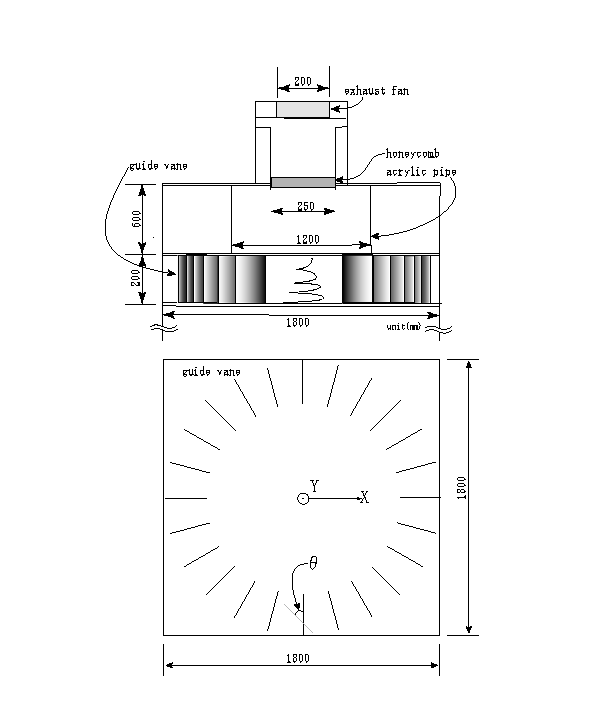
\includegraphics[width=0.8\textwidth]{./fig/matsui_tornado_generator}
\caption{龙卷风实验装置(\cite{matsui2009})}
\label{fig:matsui_tornado_generator}
\end{figure}

\begin{figure}[h!]
\centering
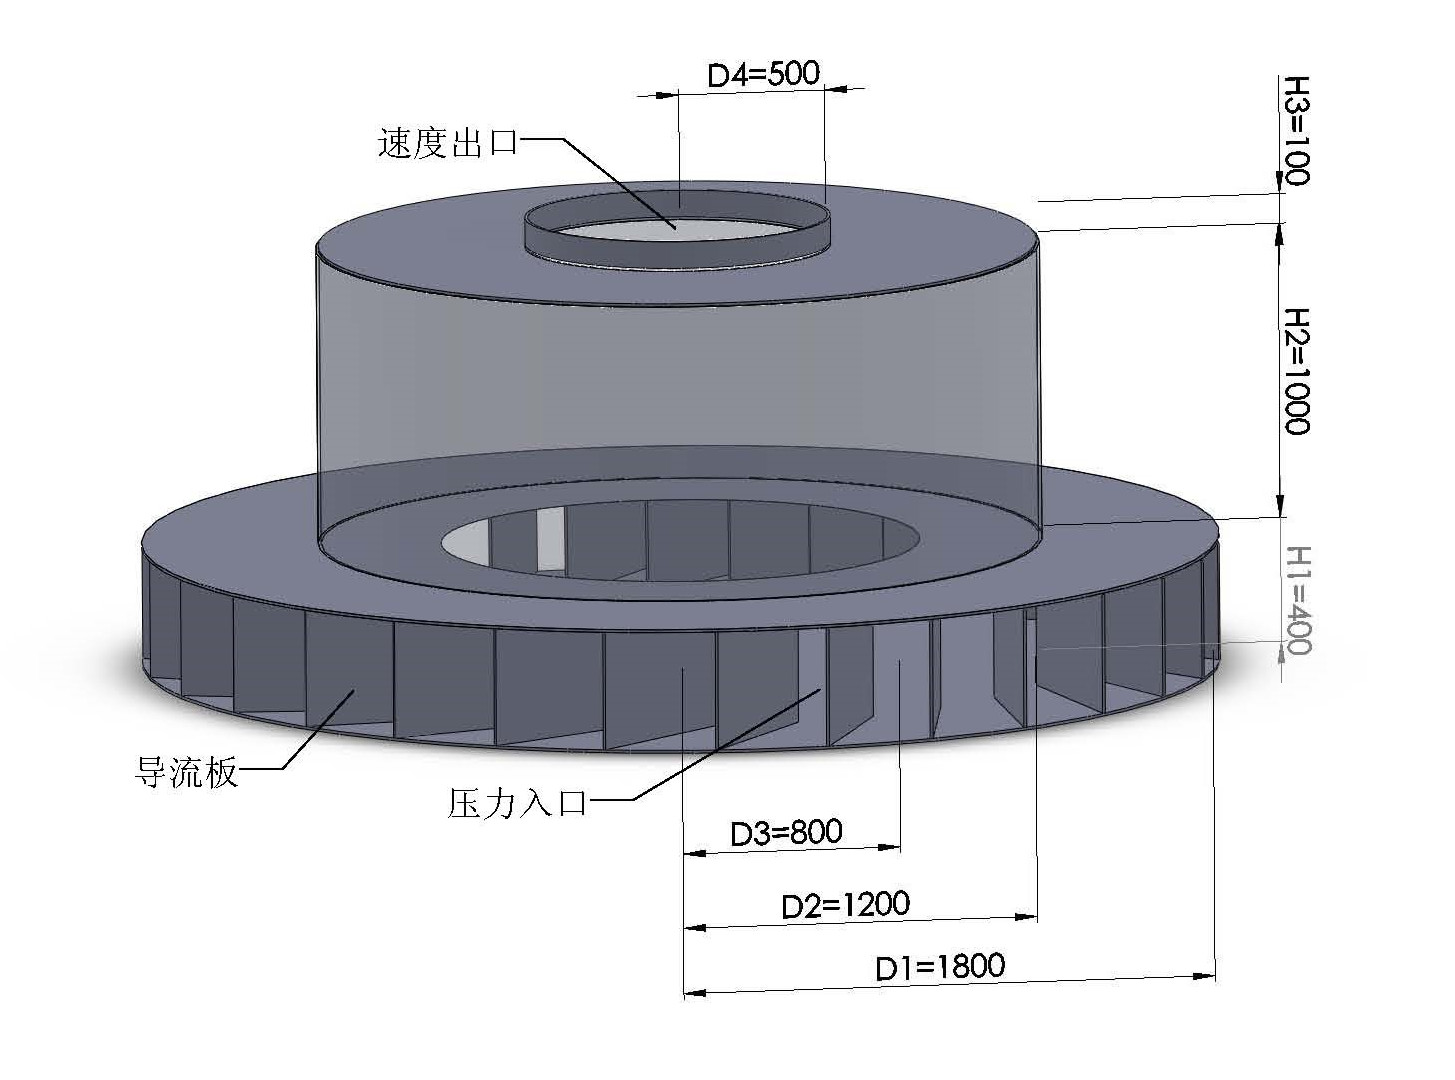
\includegraphics[width=0.9\textwidth]{./fig/tornado_generator}
\caption{龙卷风数值模拟模型}
\label{fig:tornado_generator}
\end{figure}

\begin{table}[h!]
\caption{龙卷风发生装置尺寸参数}
\label{tab:tornado_generator_parameters}
\centering
\begin{tabular*}{\textwidth}{c @{\extracolsep{\fill}} c c c c c c c}
    \toprule
   导流板角度$\theta (\SI{}{\degree})$ & $D1(\SI{}{m})$ & $D2(\SI{}{m})$ & $D3(\SI{}{m})$ & $H1(\SI{}{m})$ &  $H2(\SI{}{m})$ &  $H3(\SI{}{m})$ & 出口速度$(\SI{}{m/s})$ \\
   \midrule
   30 & 1800 & 1200 & 800 & 400 & 1000 & 100 & 52.5 \\
   \bottomrule
\end{tabular*}
\end{table}


\subsection{龙卷风的数值模型}
采用ANSYS Fluent\textregistered 计算流体力学软件对龙卷风进行数值模拟。

\subsubsection{计算区域网格的划分}
由于模型比较复杂,流域网格采用适应性良好的四面体非结构网格,如图\ref{fig:mesh}所示。

\begin{figure}[h!]
\centering
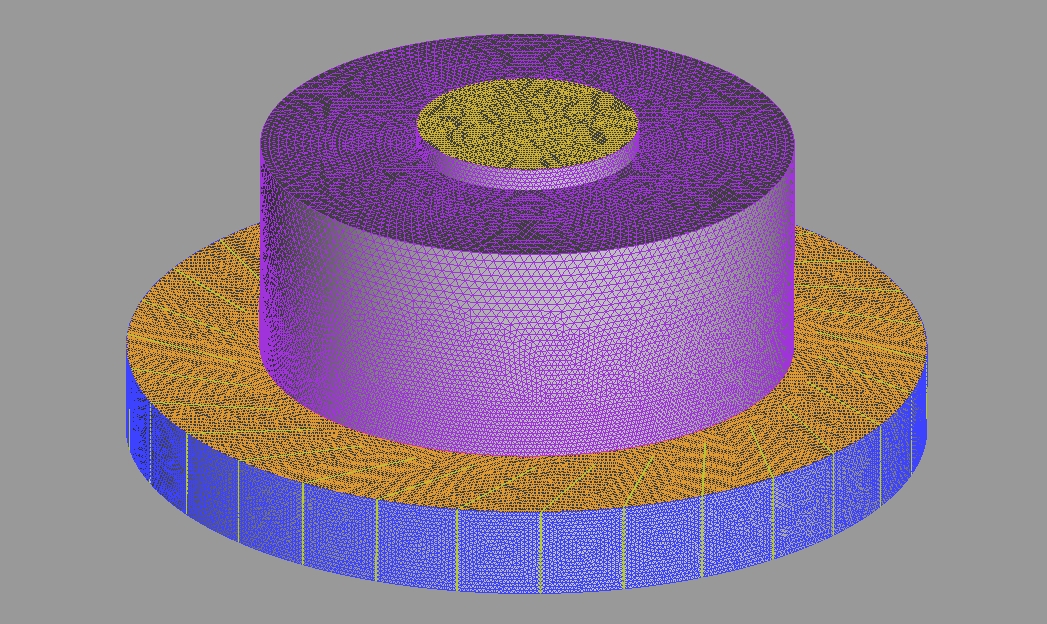
\includegraphics[width=\textwidth]{./fig/mesh}
\caption{龙卷风数值模拟的网格划分示意图}
\label{fig:mesh}
\end{figure}

由于主要关心的是近地面附近龙卷风对结构的作用,故对近地面流域处的网格进行了细分。
通过加密网格的方式,来探讨网格对计算结果的影响。
不断加密网格直到监测平面处的最大切向速度和最大切向速度所在半径的位置前后两次计算结果相差小于$5 \%$。
最后根据计算机的能力及计算结果的有效性,确定目前所采用的网格形式。

\subsubsection{湍流模型及求解设定}
本文采用三维定常计算方法,获得了龙卷风风场中各变量的时均信息。
湍流模型选取应用较广泛的RNG $k-\varepsilon$模型,近壁面采用非平衡面函数(Non-Equilibrium Wall Functions)。
离散格式采用精度较高的二阶迎风格式,离散后控制方程的求解采用压力修正的分离式解法——SIMPLEC算法。

\subsubsection{边界条件的选取}
底部入口采用压力入口(pressure-inlet),入口处的压力值与标准大气压相等;
顶部出口采用速度出口(velocity-outlet),速度方向与出口边界垂直,速度大小为\SI{52.5}{m/s};
地面、导流板以及周围筒体均采用无滑移壁面边界条件(wall)。


\subsection{数值模拟结果及正确性验证}
\subsubsection{数值模拟龙卷风的特征参数}
经软件计算,得到\SI{20}{m}高度处数值模拟龙卷风的重要特征参数如表\ref{tab:cfd_tornado_parameters}所示。
\begin{table}[h!]
\caption{数值模拟龙卷风\SI{20}{m}高度处的特征参数}
\label{tab:cfd_tornado_parameters}
\centering
\begin{tabular*}{\textwidth}{c @{\extracolsep{\fill}} c c c}
    \toprule
   龙卷风等级 & 最大旋转风速$V_{\mathrm{R}} (\SI{}{m/s})$ & 最大旋转风速半径$R(\SI{}{m})$ & 压力降$\Delta P (\SI{}{Pa})$ \\
   \midrule
   EF4 & 82.3 & 117.6 & -9841.8\\
   \bottomrule
\end{tabular*}
\end{table}

数值模拟得到的最大旋转风速为\SI{82.3}{m/s},最大旋转风速半径为\SI{117.6}{m};
而多普勒雷达测得\SI{20}{m}高度处的最大旋转风速为\SI{81.6}{m/s},最大旋转风速半径为\SI{118.6}{m}.
可见,数值模拟可较好地模拟多普勒雷达实测龙卷风的最大切向速度和最大切向速度半径。
由于本文不考虑龙卷风气压降对块状飞射物飞行的影响,故不再验证数值龙卷风模型的气压降。

\subsubsection{切向速度的分布特征}
图\ref{fig:Vr}为\SI{20}{m}高度处龙卷风的切向速度随其半径的变化曲线图,包括:
\SI{20}{m}高度处数值龙卷风模拟结果,Rankine涡模型结果及美国南达科他州Spencer地区实际发生龙卷风\SI{20}{m}高度处的多普勒雷达实测结果。

\begin{figure}
\centering
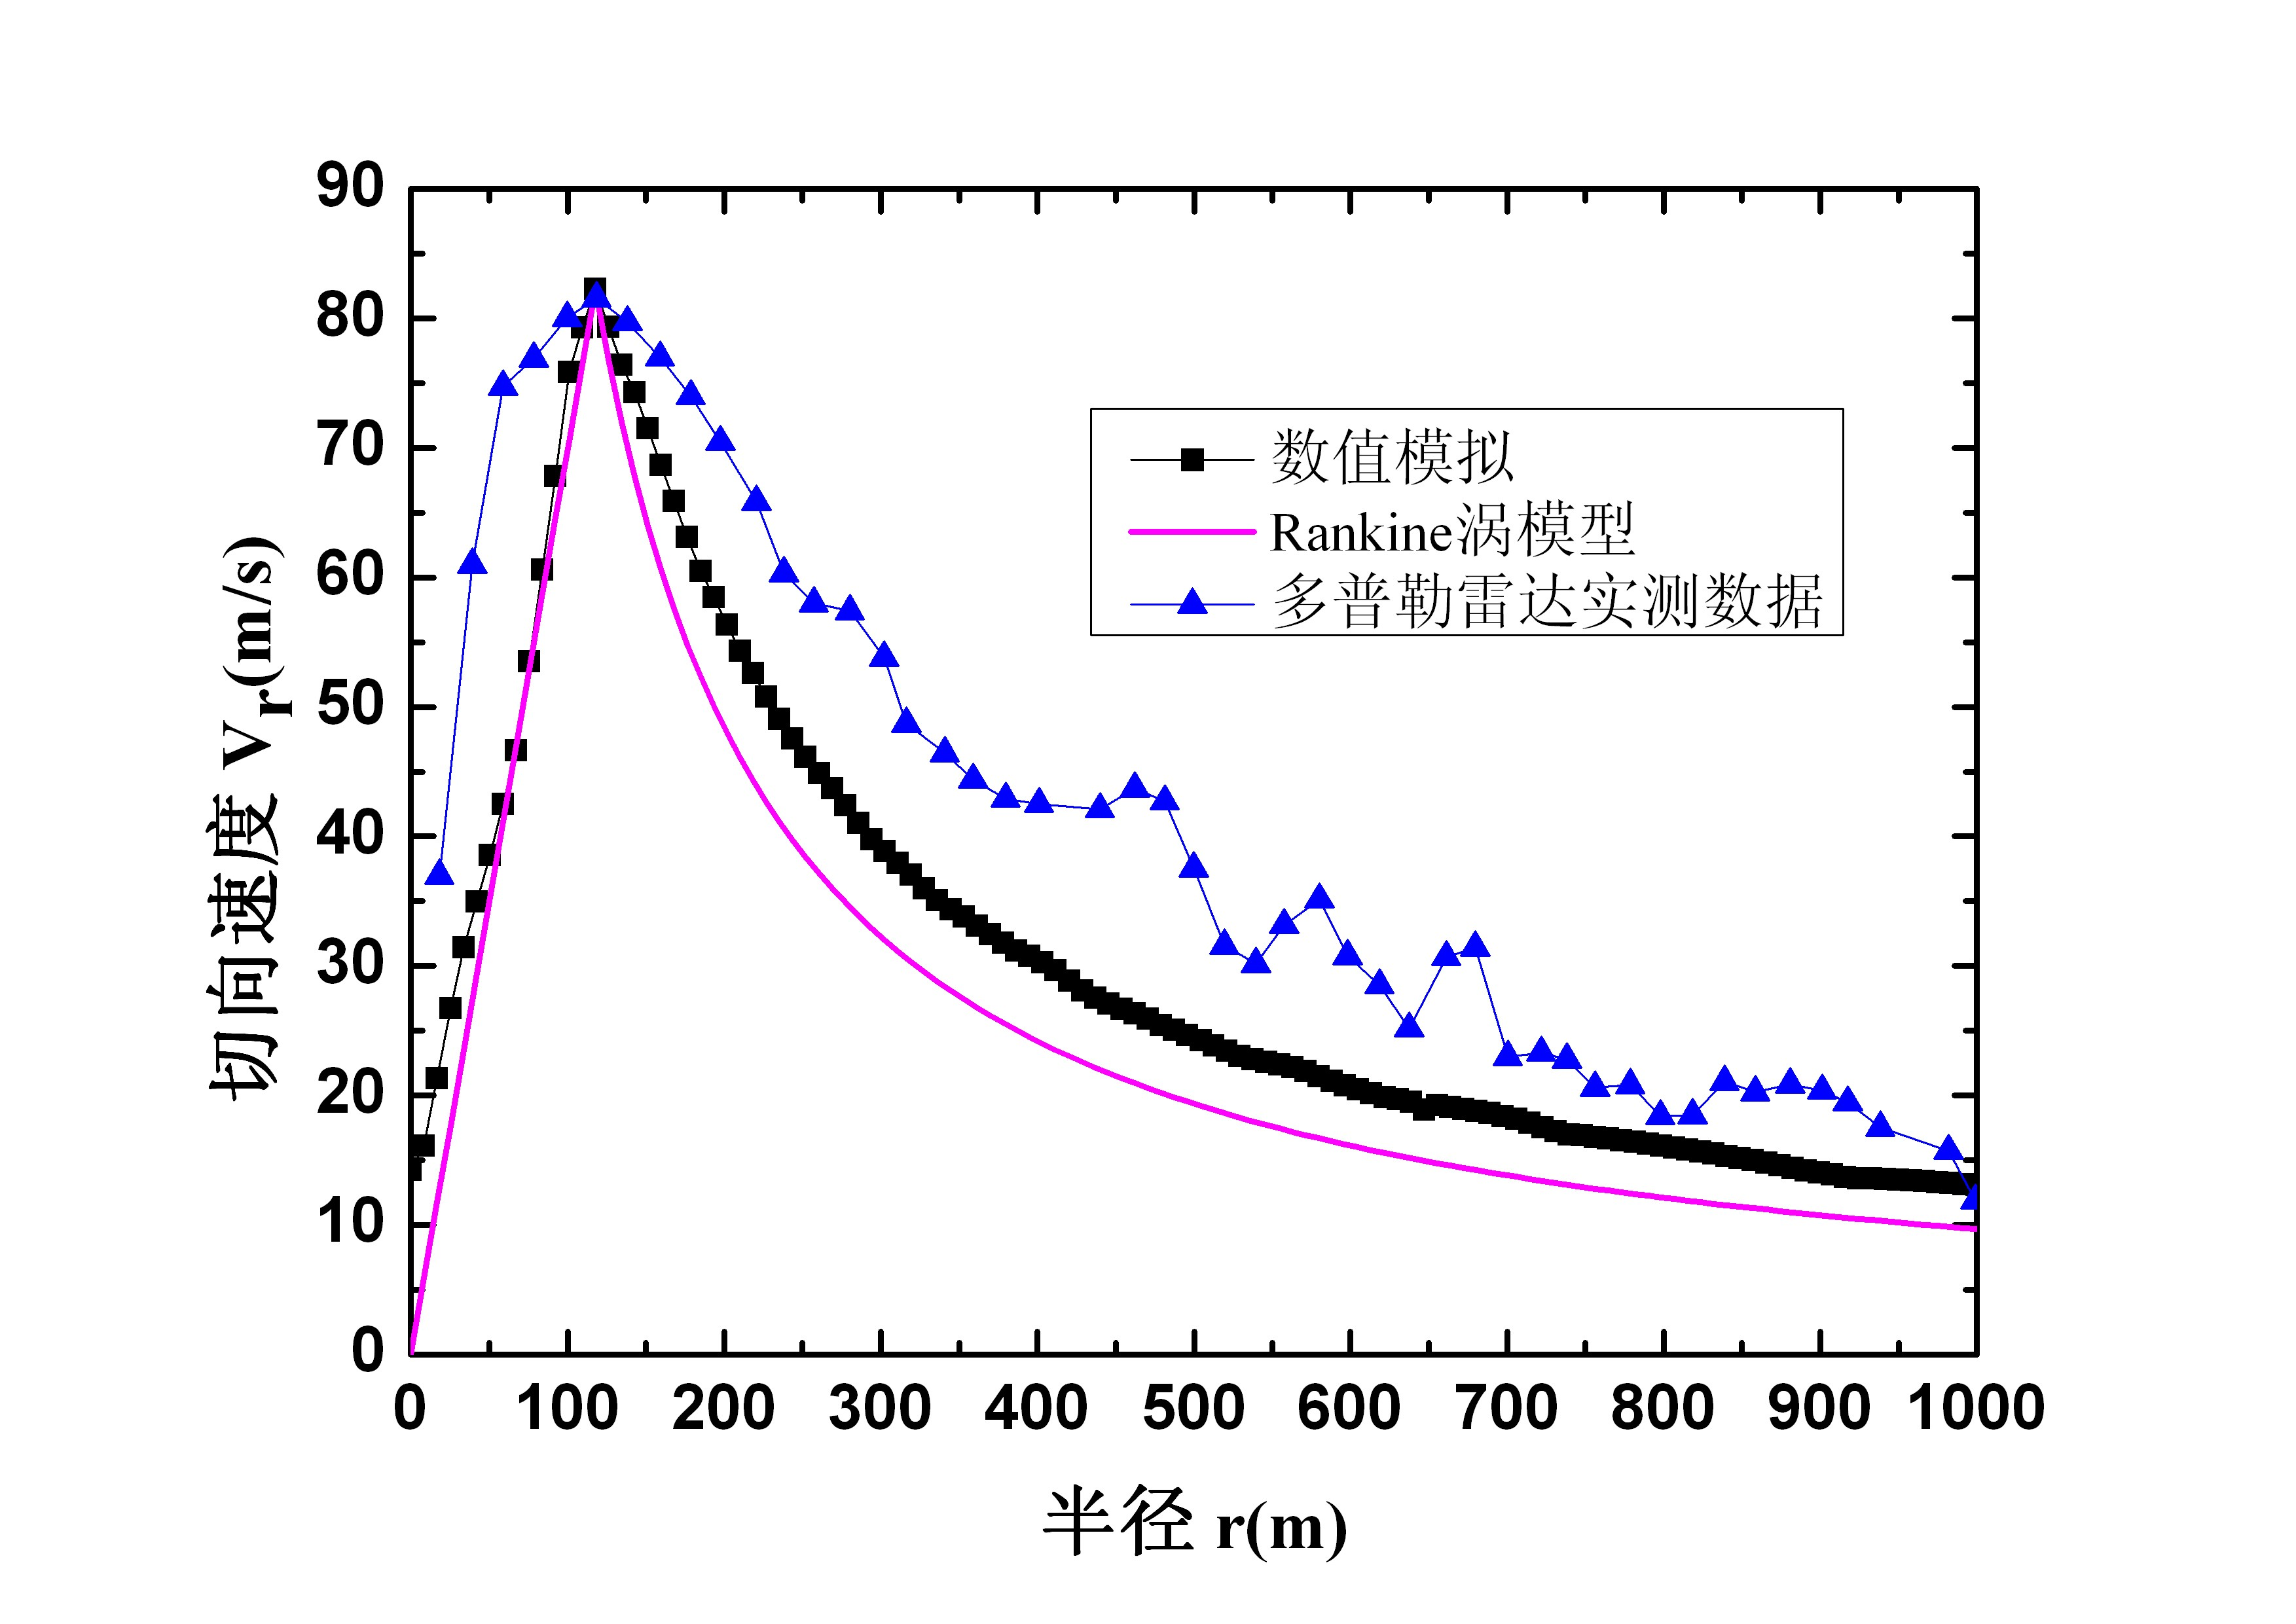
\includegraphics[width=0.8\textwidth]{./fig/Vr}
\caption{\SI{20}{m}高度处龙卷风切向速度随半径变化示意图}
\label{fig:Vr}
\end{figure}


从图中可以看出,Rankine涡模型和数值模拟的结果都较好地模拟了美国南达科他州Spencer地区实际发生的龙卷风,能反映出龙卷风切向速度随其半径的变化规律。
实际情况中,龙卷风是非定常,雷达观测到的数据是通过时间平均得到的。
本文数值模拟方法假定龙卷风是定常的,利用固定的边界条件和初始条件模拟了定常的龙卷风涡结构,与实际的龙卷风略有不同。
并且本文数值模拟方法采用的是均匀沙粒状的地表面,与实际地面粗糙度可能并不一致,从而导致摩擦力的影响有所不同,而Rankine涡模型甚至没有考虑摩擦力的影响。
由于这些偏差的存在,使得数值模拟结果不可能完全与Rankine涡模型以及雷达观测的数据一致。




\printbibliography
\end{document}